\chapter{Diseños individuales para la iteración competitiva de Álvaro Gómez Sittima}
\label{ape:disenyoAlvaro}
En este apéndice se muestran los diseños individuales realizados por Álvaro Gómez Sittima para la iteración competitiva. En la Figura \ref{fig:disenyoAlvaro01} se muestra el diseño de la pantalla de inicio, tanto con un archivo PDF como sin él. En la Figura \ref{fig:disenyoAlvaro02} se presenta la funcionalidad de generar resumen. En la Figura \ref{fig:disenyoAlvaro03} se muestra el diseño de la funcionalidad de pictotraductor. En la Figura \ref{fig:disenyoAlvaro04} se muestra el diseño del ejercicio de completar huecos. En la Figura \ref{fig:disenyoAlvaro05} se presenta la funcionalidad de buscar pictogramas. Finalmente, en la Figura \ref{fig:disenyoAlvaro06} se muestra el diseño de la funcionalidad de crear ejercicios de definiciones.

\begin{figure}[h!]
  \centering
  \begin{subfigure}{\textwidth}
    \centering
    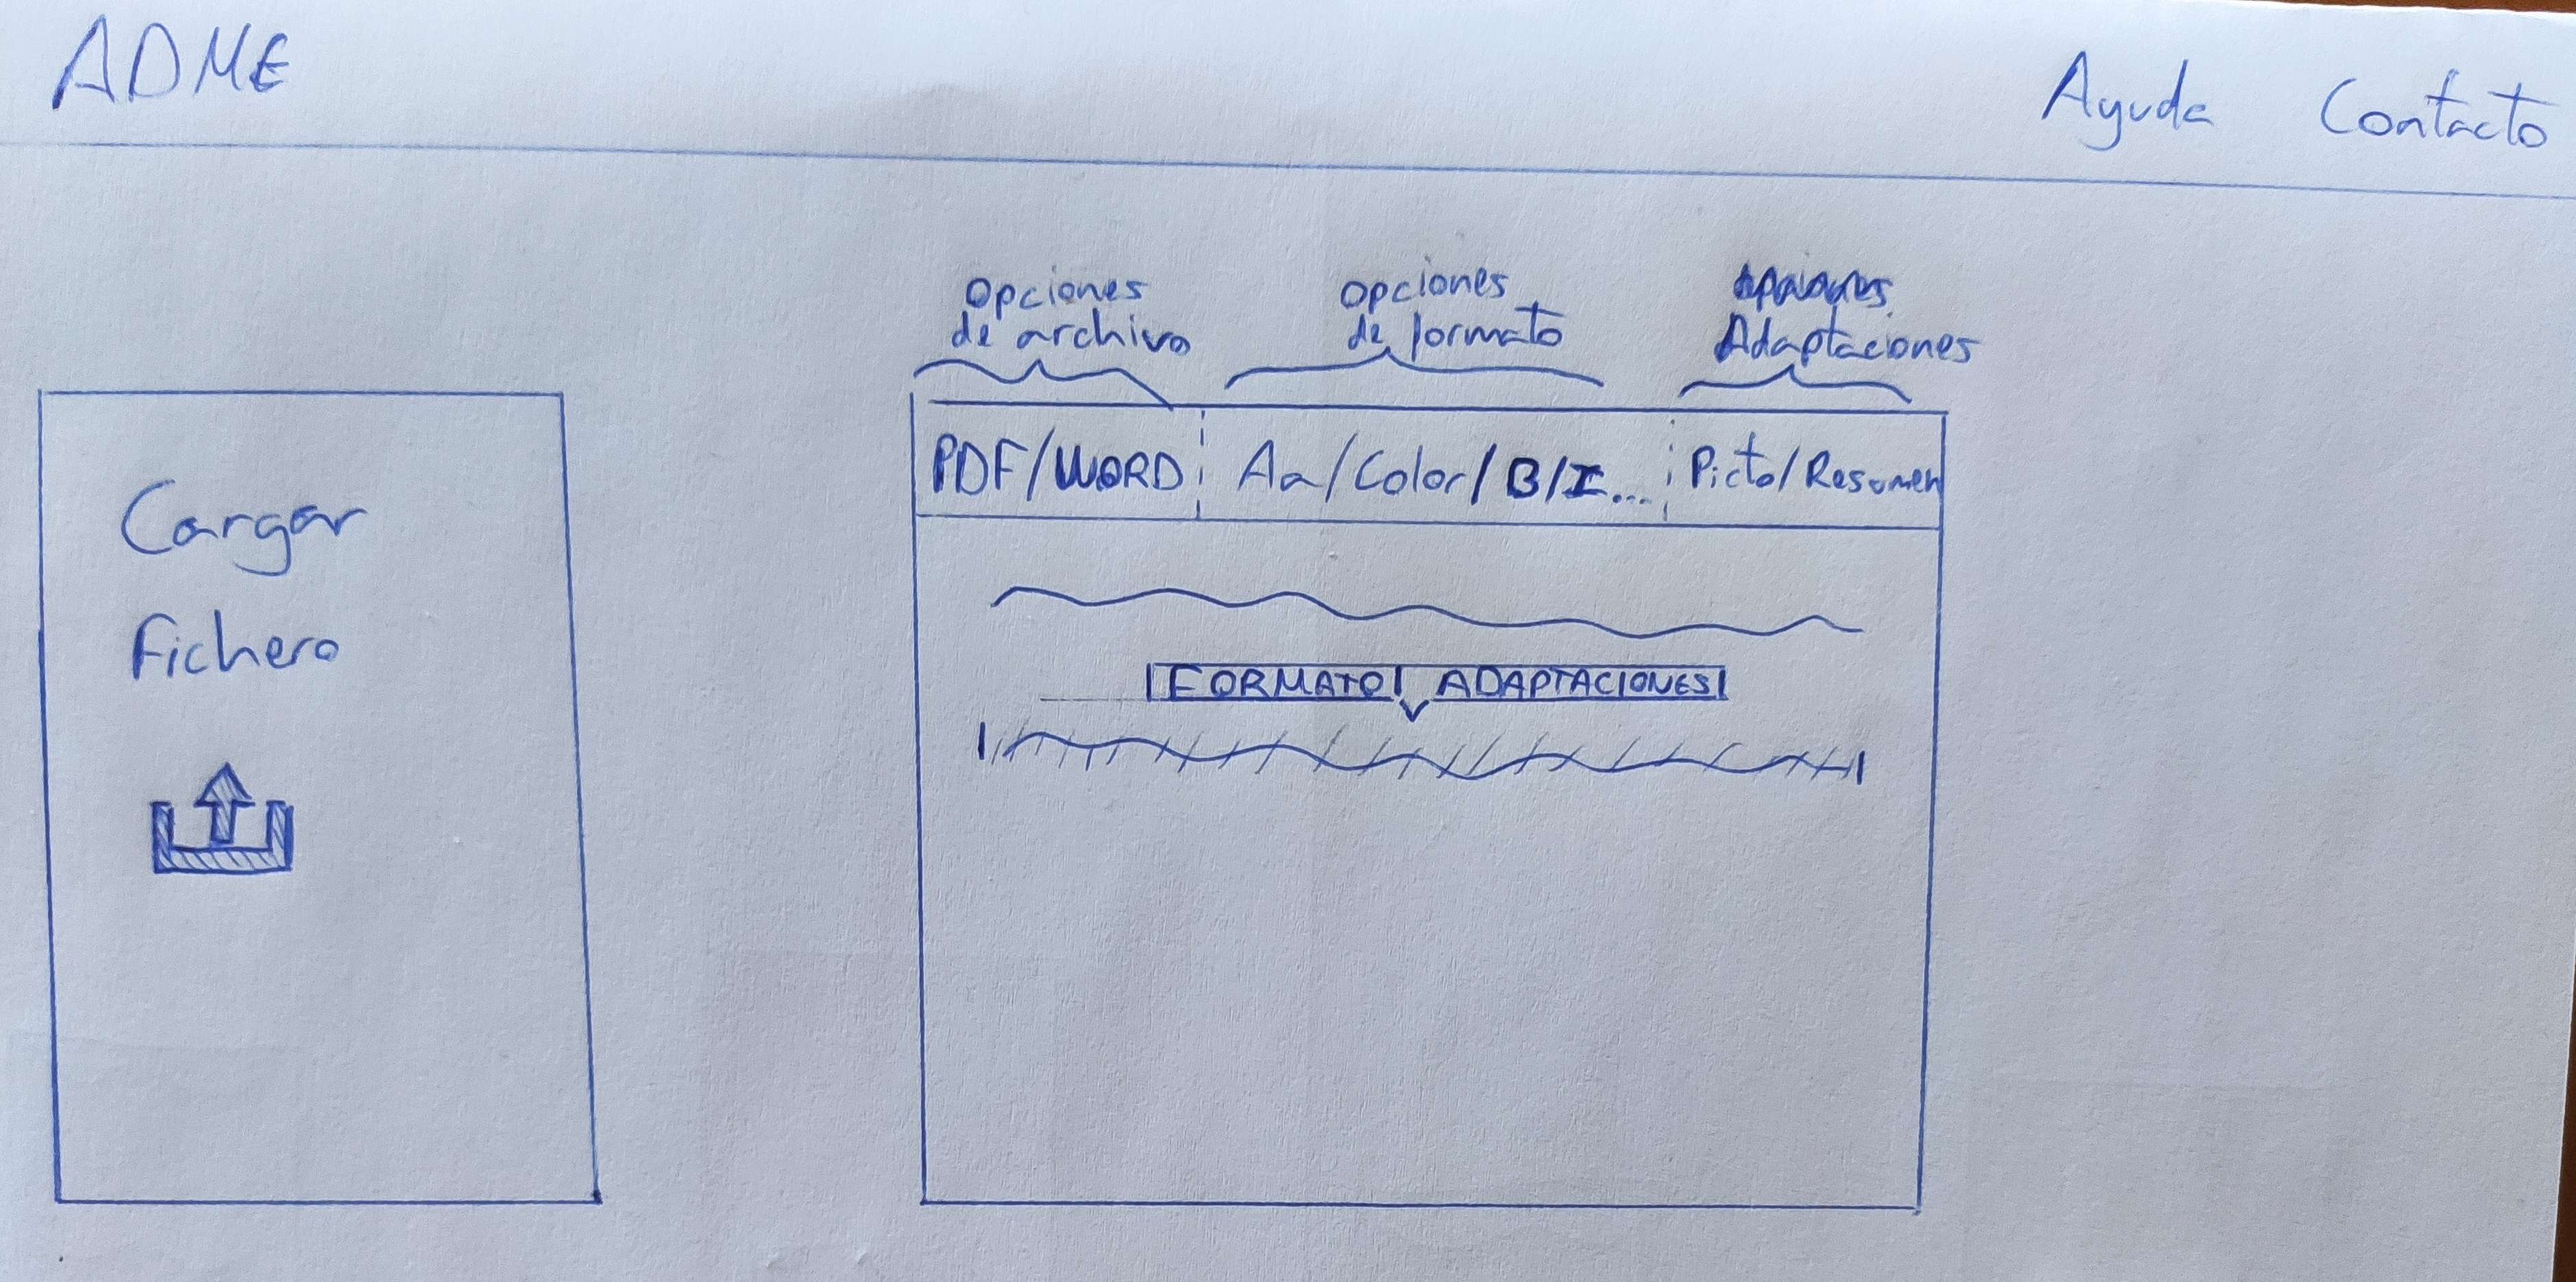
\includegraphics[width=0.55\textwidth]{Diseño/Alvaro/Alvaro01.jpg}
    \caption{Página de inicio sin PDF.}
    \label{fig:disenyoAlvaro01a}
  \end{subfigure}
  \begin{subfigure}{\textwidth}
    \centering
    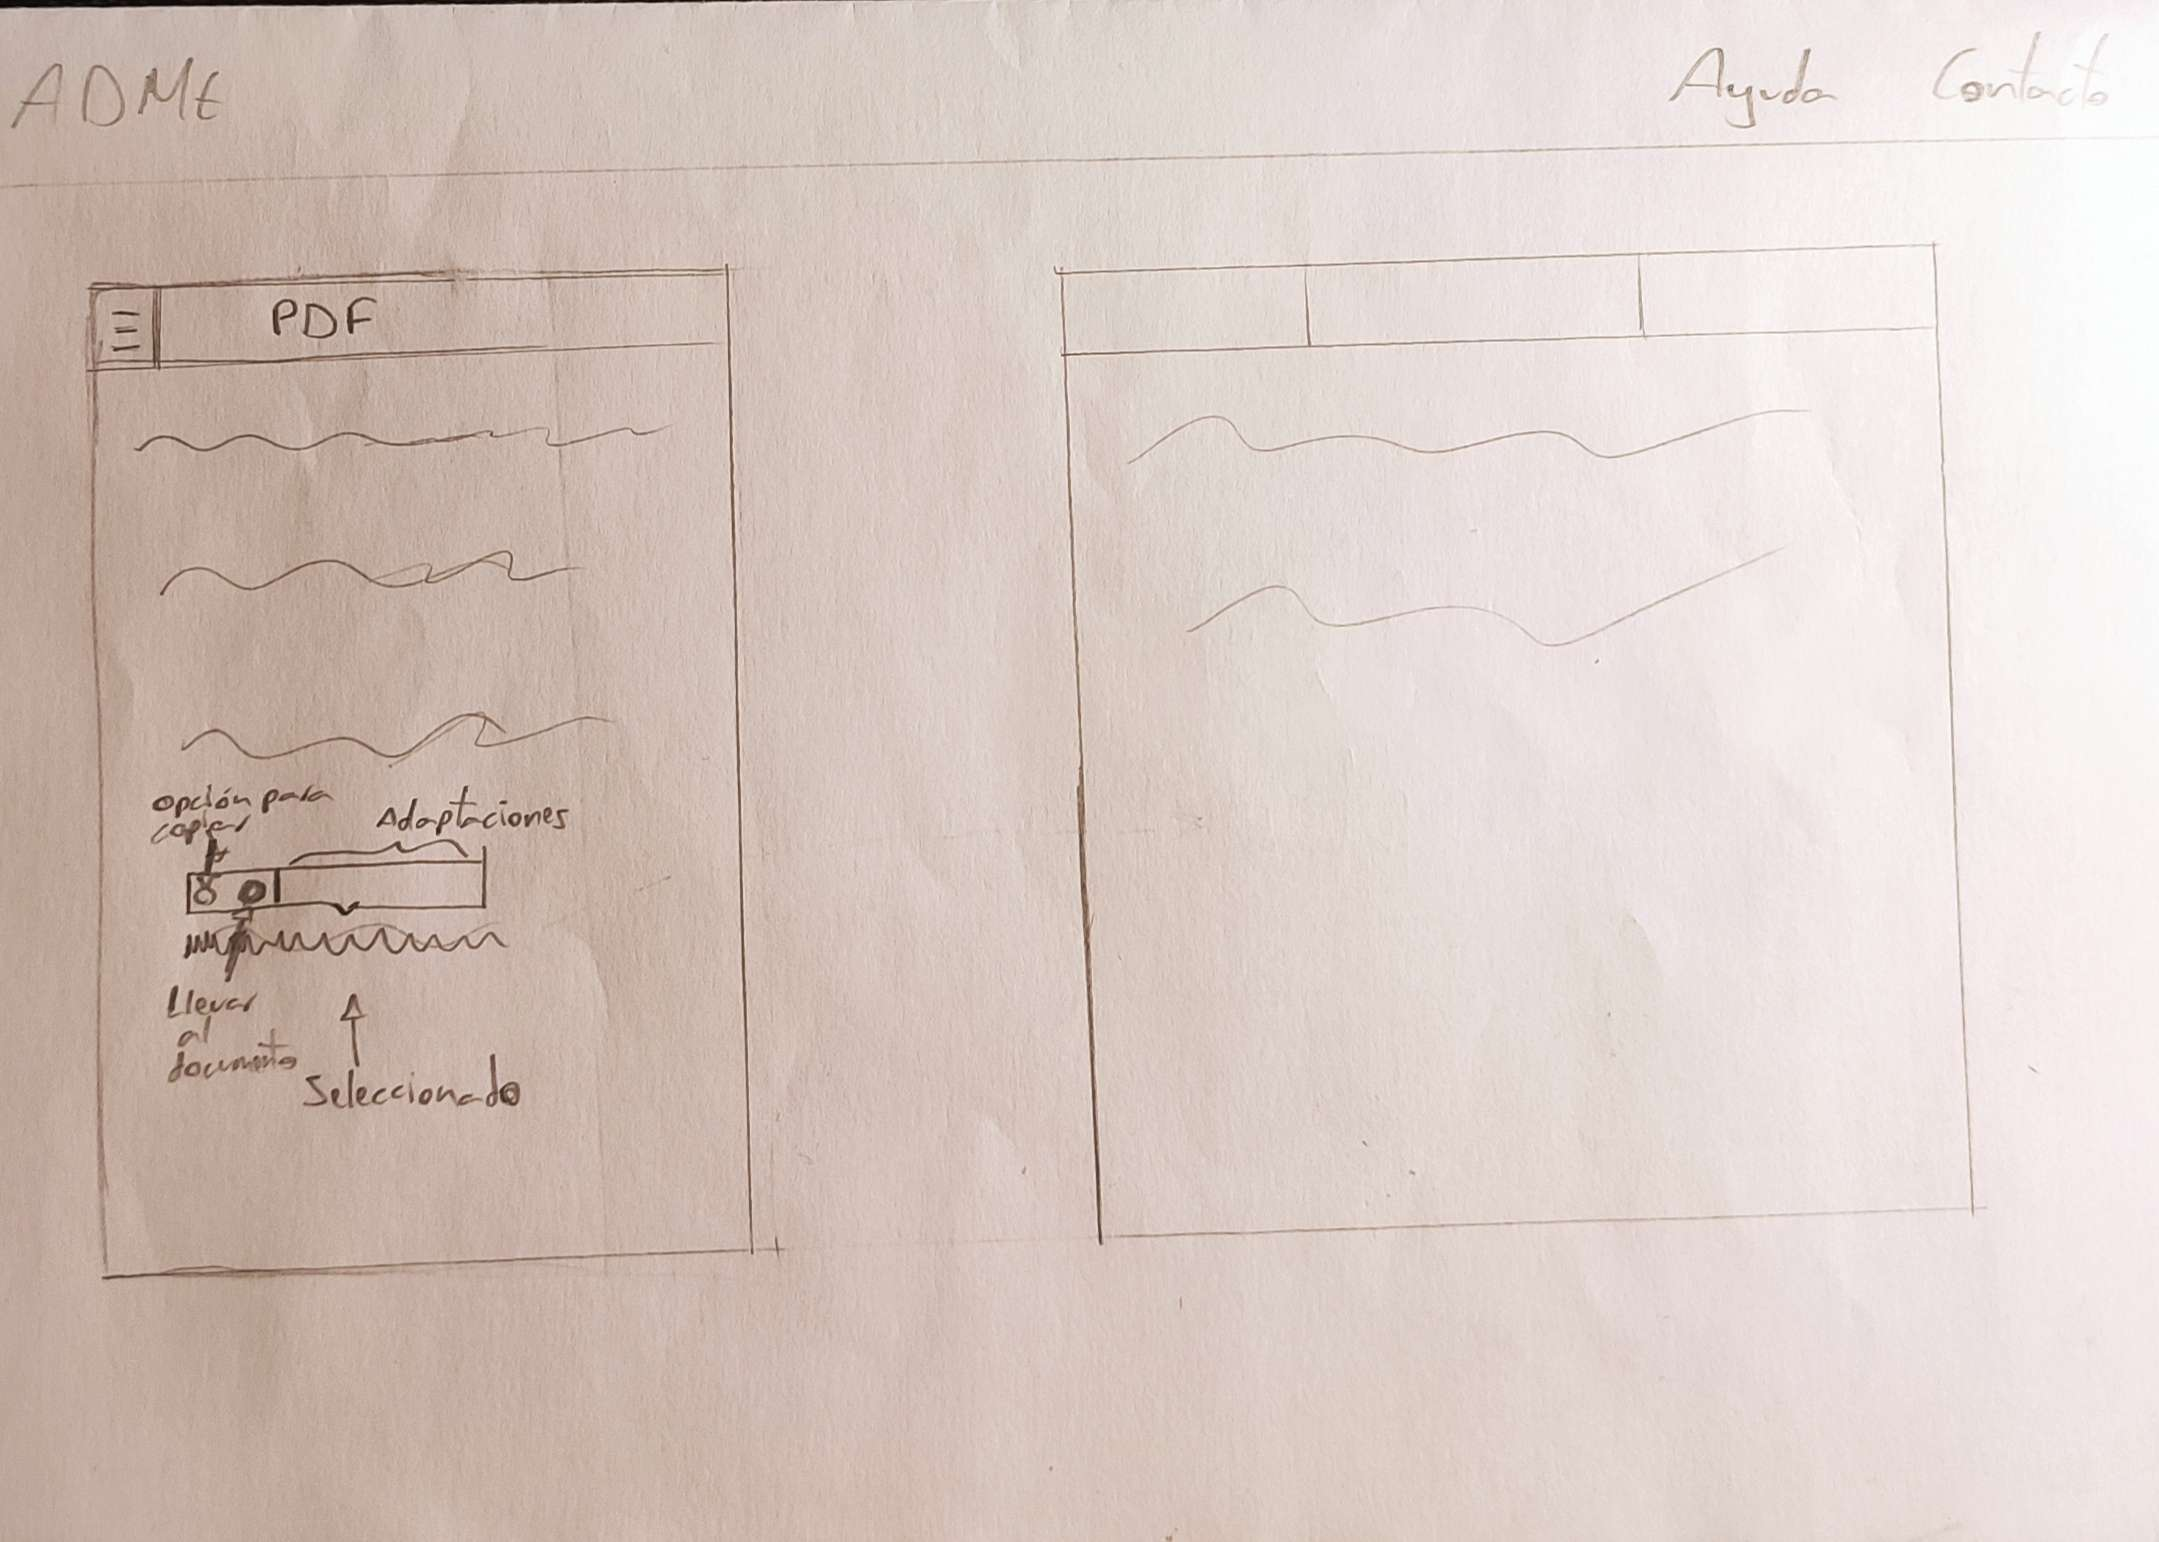
\includegraphics[width=0.55\textwidth]{Diseño/Alvaro/Alvaro02.jpg}
    \caption{Página de inicio con PDF.}
    \label{fig:disenyoAlvaro01b}
  \end{subfigure}

  \caption{Diseño de la página de inicio de Álvaro.}
  \label{fig:disenyoAlvaro01}
\end{figure}

\begin{figure}[ht!]
  \centering
  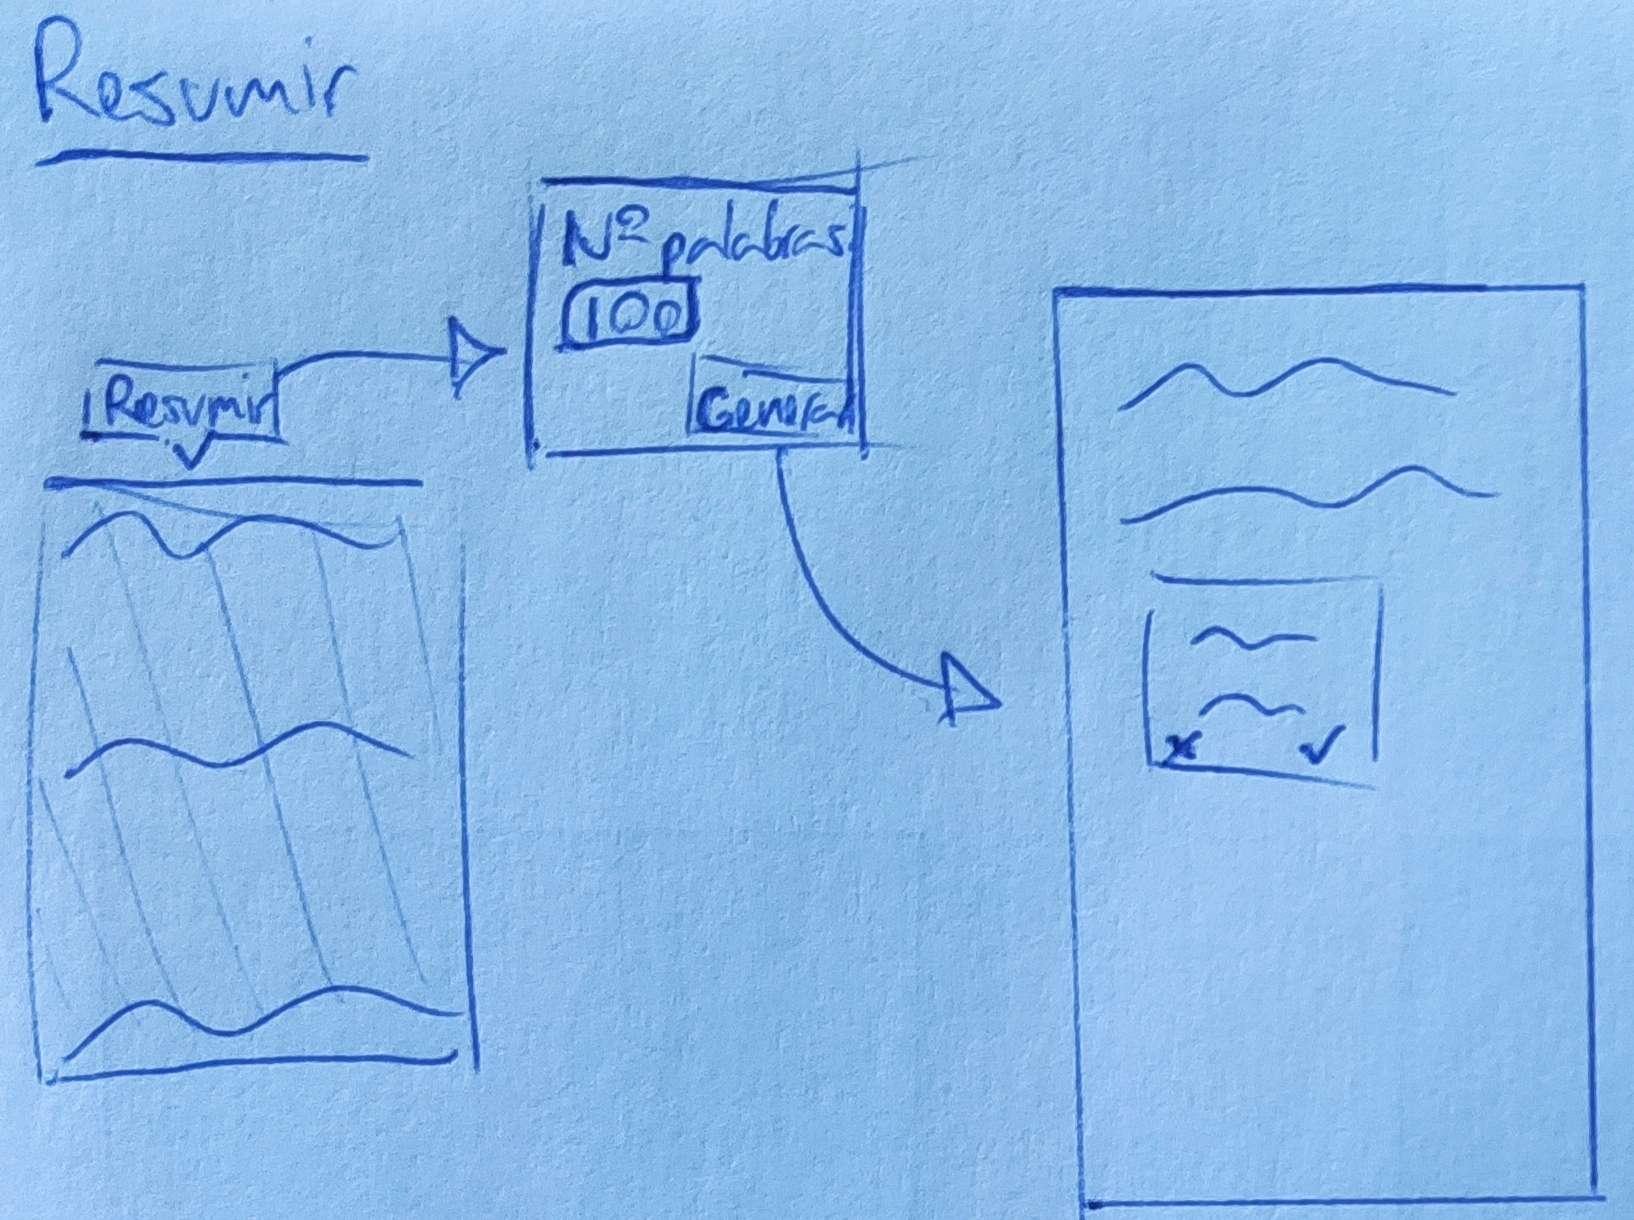
\includegraphics[width=0.65\textwidth]{Diseño/Alvaro/Alvaro03.jpg}
  \caption{Diseño de generar resumen de Álvaro.}
  \label{fig:disenyoAlvaro02}
\end{figure}

\begin{figure}[ht!]
  \centering
  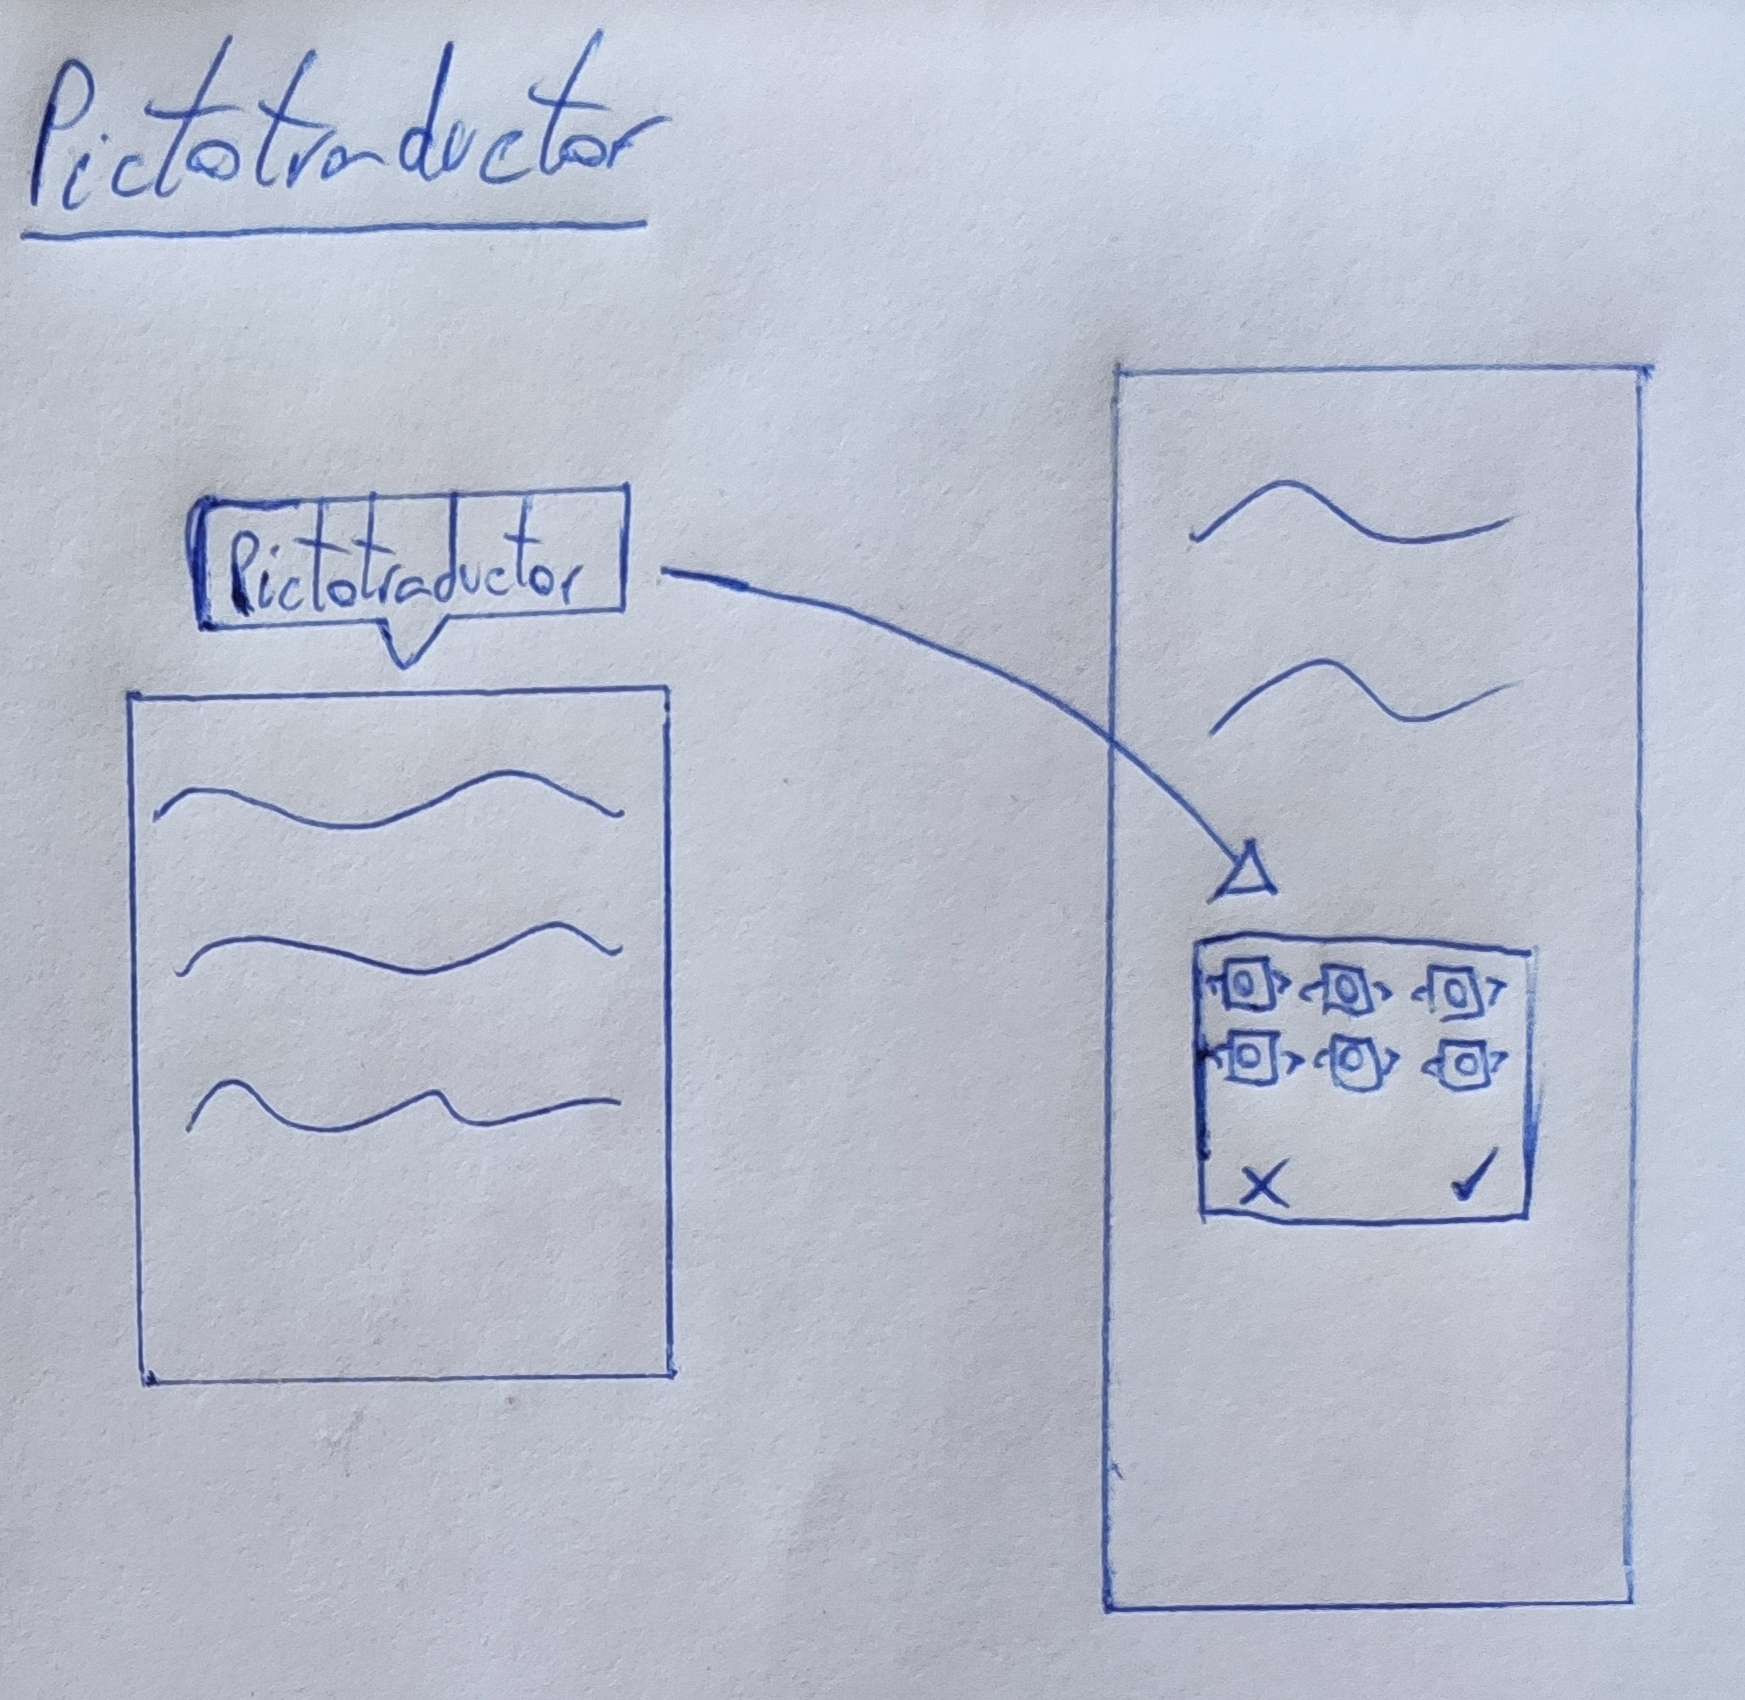
\includegraphics[width=0.65\textwidth]{Diseño/Alvaro/Alvaro04.jpg}
  \caption{Diseño de pictotraductor de Álvaro.}
  \label{fig:disenyoAlvaro03}
\end{figure}

\begin{figure}[ht!]
  \centering
  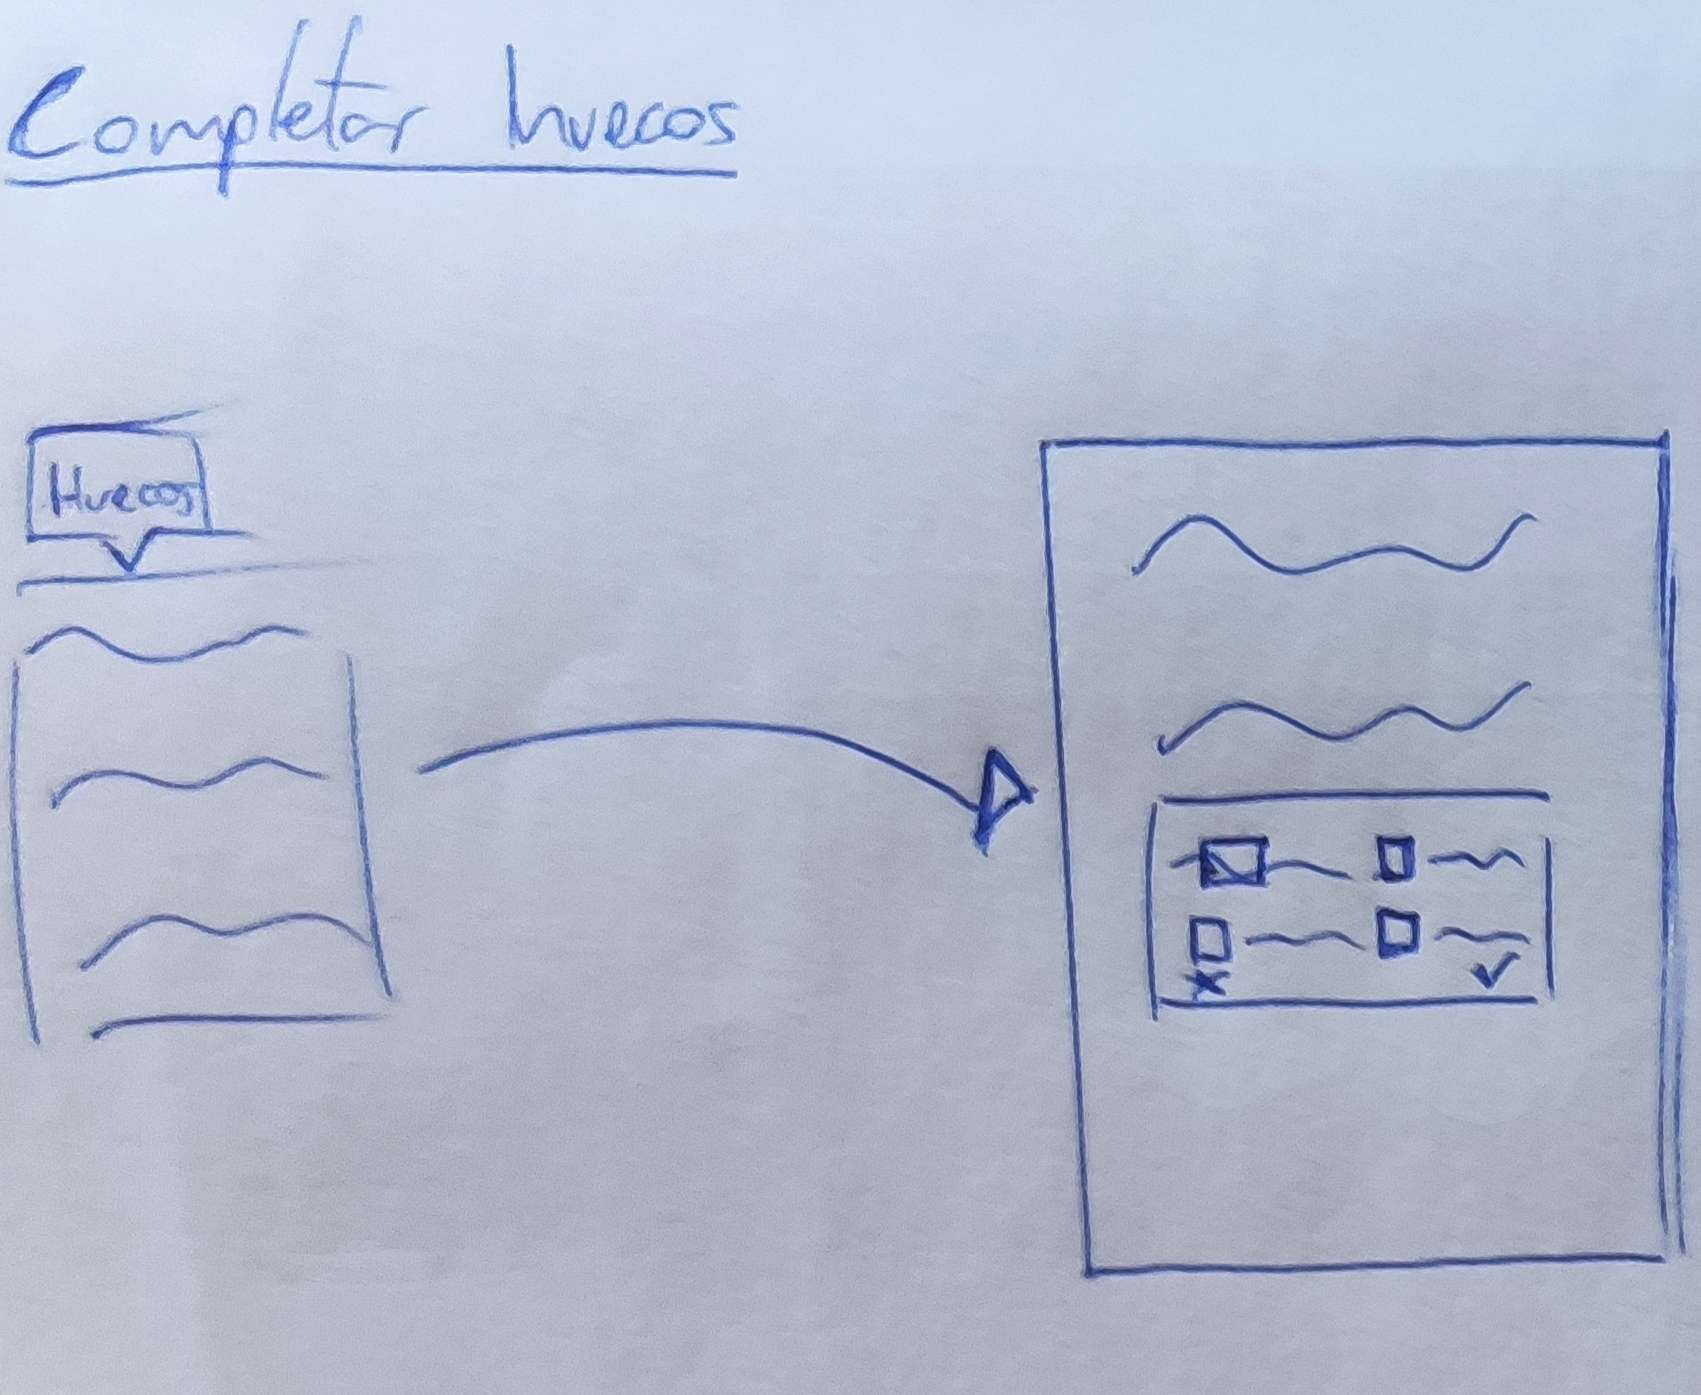
\includegraphics[width=0.65\textwidth]{Diseño/Alvaro/Alvaro05.jpg}
  \caption{Diseño de definir huecos de Álvaro.}
  \label{fig:disenyoAlvaro04}
\end{figure}

\begin{figure}[ht!]
  \centering
  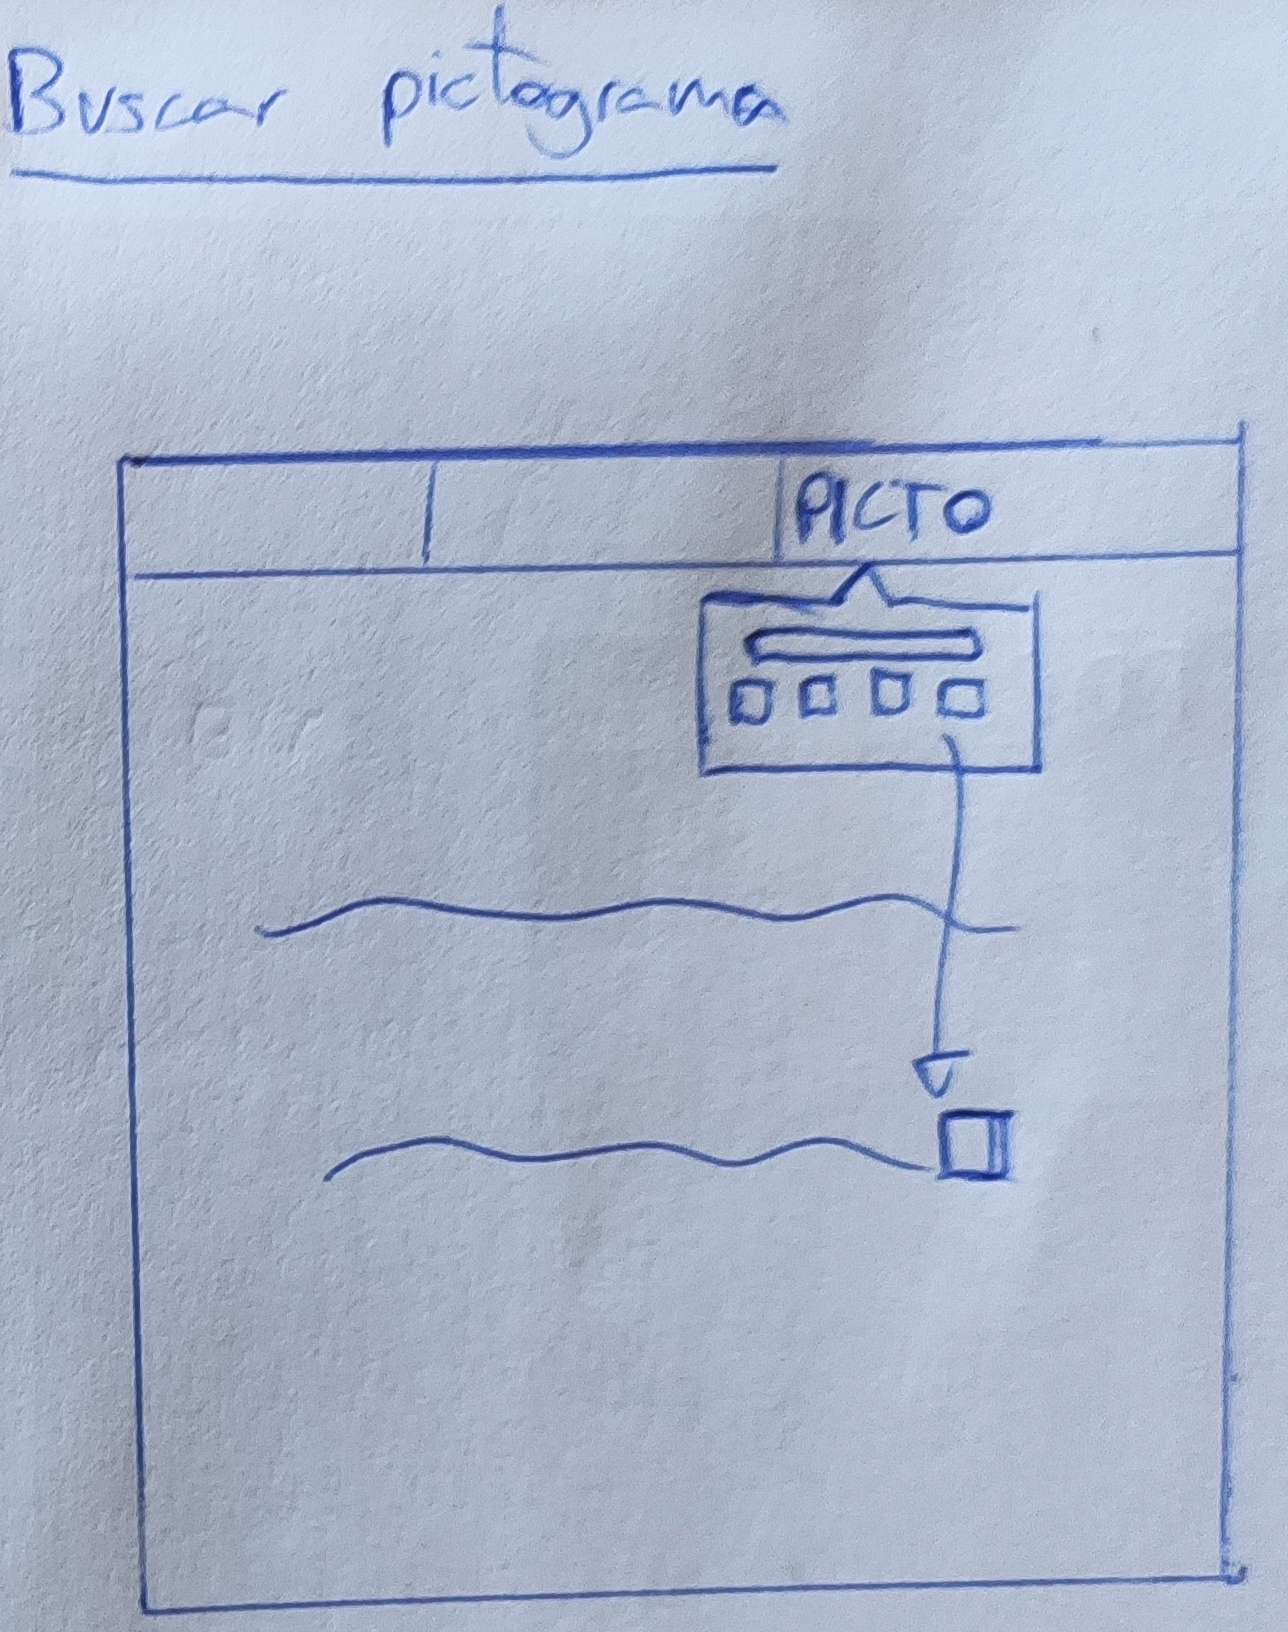
\includegraphics[width=0.65\textwidth]{Diseño/Alvaro/Alvaro06.jpg}
  \caption{Diseño de buscar pictogramas de Álvaro.}
  \label{fig:disenyoAlvaro05}
\end{figure}

\begin{figure}[ht!]
  \centering
  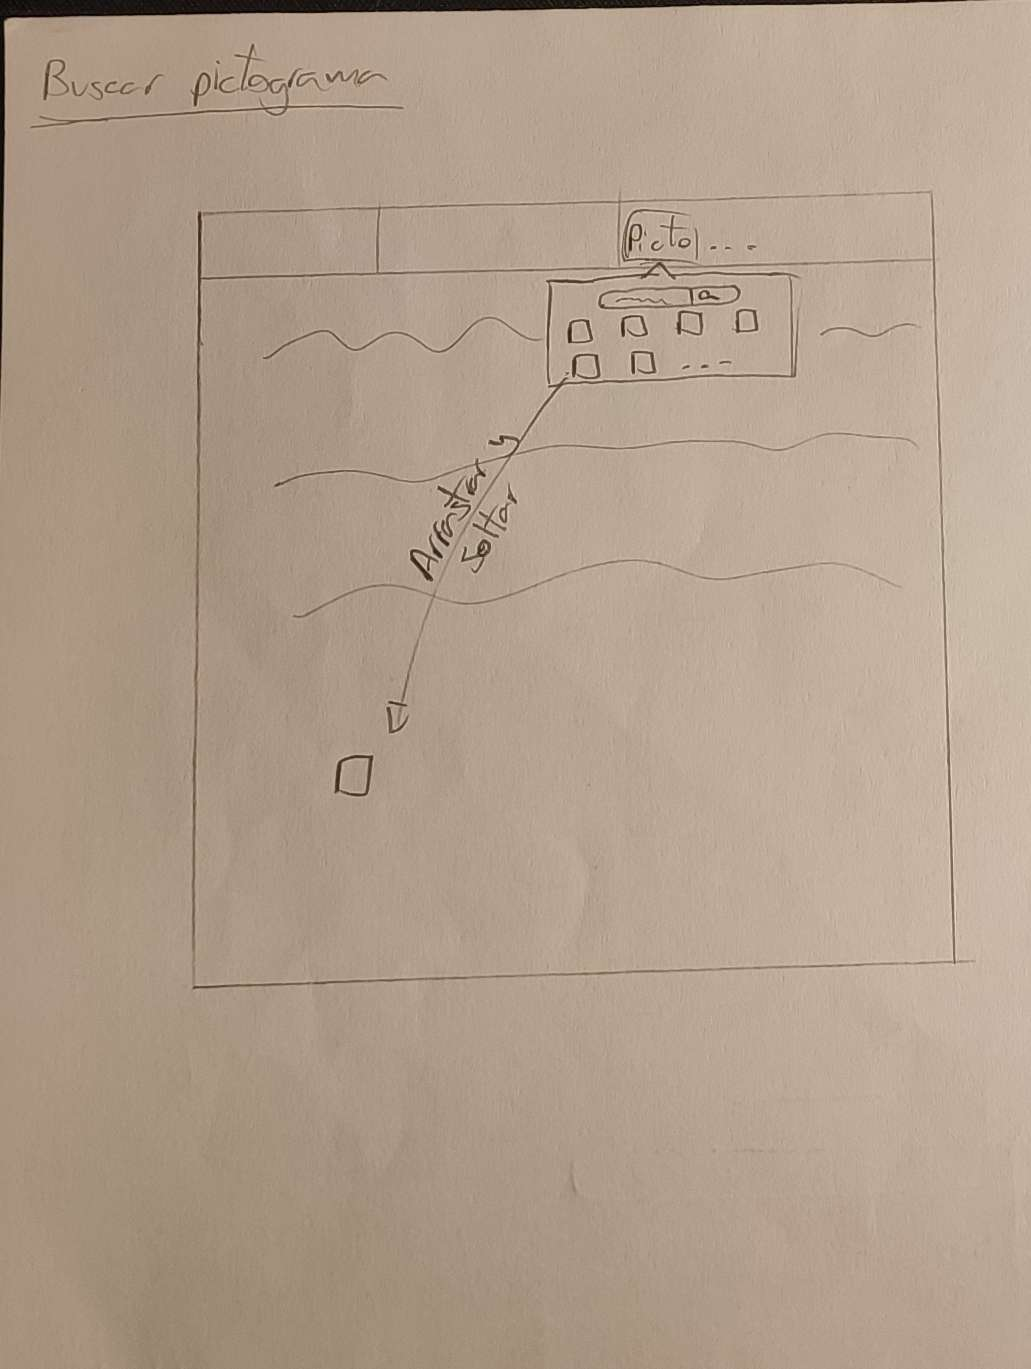
\includegraphics[width=0.7\textwidth]{Diseño/Alvaro/Alvaro07.jpg}
  \caption{Diseño de ejercicio de definiciones de Álvaro.}
  \label{fig:disenyoAlvaro06}
\end{figure}